\documentclass[12pt, hidelinks]{article}
\usepackage[brazil]{babel}
\usepackage[utf8]{inputenc}
\usepackage{amsmath}
\usepackage{natbib}
\usepackage{listings}
\usepackage{color}

\definecolor{codegreen}{rgb}{0,0.6,0}
\definecolor{codegray}{rgb}{0.5,0.5,0.5}
\definecolor{codepurple}{rgb}{0.58,0,0.82}
\definecolor{backcolour}{rgb}{0.95,0.95,0.92}

\lstdefinestyle{mystyle}{
  backgroundcolor=\color{backcolour},
  commentstyle=\color{codegreen},
  keywordstyle=\color{red},
  numberstyle=\tiny\color{codegray},
  stringstyle=\color{codepurple},
  basicstyle=\footnotesize,
  breakatwhitespace=false,
  breaklines=true,
  captionpos=b,
  keepspaces=true,
  numbers=left,
  numbersep=5pt,
  showspaces=false,
  showstringspaces=false,
  showtabs=false,
  tabsize=2,
  extendedchars=true,
  literate={á}{{\'a}}1 {ã}{{\~a}}1 {õ}{{\~o}}1 {é}{{\'e}}1 {ç}{{\c{c}}}1,
}

\lstset{style=mystyle}
\usepackage{url}
\usepackage{amsmath}
\usepackage{float}
\usepackage{graphicx}
\graphicspath{{images/}}
\usepackage{parskip}
\usepackage{fancyhdr}
\usepackage{vmargin}
\usepackage{hyperref}
\setmarginsrb{3 cm}{2.5 cm}{3 cm}{2.5 cm}{1 cm}{1.5 cm}{1 cm}{1.5 cm}


\title{Ajuste de Curvas}								% Title
\author{Wilton Rodrigues}								% Author
\date{\today}											% Date

\makeatletter
\let\thetitle\@title
\let\theauthor\@author
\let\thedate\@date
\makeatother

\pagestyle{fancy}
\fancyhf{}
\lhead{\centering{\thetitle}}
\cfoot{\thepage}

\begin{document}

%%%%%%%%%%%%%%%%%%%%%%%%%%%%%%%%%%%%%%%%%%%%%%%%%%%%%%%%%%%%%%%%%%%%%%%%%%%%%%%%%%%%%%%%%

\begin{titlepage}
  \centering
  \begin{figure}[H]
    \centering
    
\includegraphics[width=0.7\textwidth]{figuras/logo.png}\\[2.0 cm]
  \end{figure}
  \textsc{\LARGE Universidade de Brasília}\\[2.5 cm]	% University Name
  \textsc{\Large Relatório de atividade do módulo 3}\\[0.5 cm]				% Activity name
  \textsc{\large Métodos Numéricos para Engenharia}\\[1.5 cm]				% Course Name
  \rule{\linewidth}{0.2 mm} \\[0.4 cm]
  {\huge \bfseries \thetitle}\\
  \rule{\linewidth}{0.2 mm} \\[2.5 cm]

  \begin{minipage}{0.4\textwidth}
    \begin{flushleft} \large
      \emph{Aluno:}\\
      \theauthor
    \end{flushleft}
  \end{minipage}
  \begin{minipage}{0.4\textwidth}
    \begin{flushright} \large
      \emph{Matrícula:} \\
      13/0049212									% Your Student Number
    \end{flushright}
  \end{minipage}\\
  \vspace*{0.5in}
  {\large \thedate}\\[0.5 cm]

  \vfill

\end{titlepage}

%%%%%%%%%%%%%%%%%%%%%%%%%%%%%%%%%%%%%%%%%%%%%%%%%%%%%%%%%%%%%%%%%%%%%%%%%%%%%%%%%%%%%%%%%

\section{Introdução}

O objetivo deste relatório é exercitar os conceitos aprendidos em aula, com relação ao tópico: \thetitle.
Que tem como objetivo prover métodos matemáticos capazes de prover soluções para situações em que conhece-se
uma tabela de pontos $(x_i, y_i)$, onde cada $y_i$ é obtido experimentalmente, e deseja-se obter a expressão
analítica de uma dada curva $y = f(x)$ que melhor se ajusta a esse conjunto de pontos.
O problema a ser solucionado é o que trata de placas de orifício com bordas em canto, que são utilizadas na
medição da vazão de fluídos através de tubulações.

\begin{figure}[!h]
  \centering
  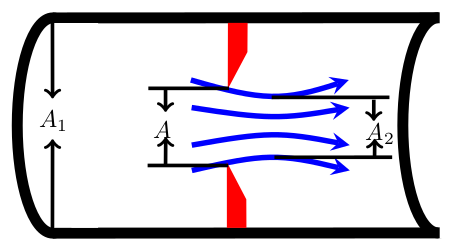
\includegraphics[width=5cm]{figuras/problema.png}\\
  \caption{Placa de orifício com bordas em canto}\label{fig:placa}
\end{figure}

A figura acima mostra uma placa de orifício que tem os seguintes parâmetros representativos: a área $A$ da
seção reta do orifício, a área $A_L$ da seção reta da tubulação e $A_2$ = $CA$ que é a seção reta no ponto de maior
concentração após o orifício. O coeficiente $C$ está em função da vazão $\dfrac{A}{A_1}$, e os valores, obtidos experimentalmente,
estão na tabela abaixo:

\begin{table}[h]
  \centering
  \vspace{0.5cm}
  \begin{tabular}{|r|r|r|r|r|r|r|r|r|r|r|}
    \hline
      $\frac{A}{A_1} = x_i$ & 0.10 & 0.20 & 0.30 & 0.40 & 0.50 & 0.60 & 0.70 & 0.80 & 0.90 & 1.00\\
    \hline
      $C = y_i$ & 0.62 & 0.63 & 0.64 & 0.66 & 0.68 & 0.71 & 0.76 & 0.81 & 0.89 & 1.00\\
    \hline
  \end{tabular}
  \caption{Valores experimentais}
\end{table}

A solução do problema se dará fazendo $x = \dfrac{A}{A_1}$, aproximando a função $C(x)$ pela função $a_0 + a_1x + a_2x^2$ utilizando
o método dos mínimos quadrados e solucionando o sistema resultante pelo método de eliminação de Gauss-Jordan. Além de apresentar um
gráfico do polinômio obtido e dos pontos da tabela, e comparando os valores do polinômio com os valores da tabela.

\section{Metodologia}

Baseando-se no método dos mínimos quadrados, primeiramente iremos organizar nossos dados experimentais de acordo com a notação exigida pelo
método. Que para uma função polinomial de grau 2 fica da seguinte maneira:
\begin{eqnarray}\label{eq:matrizes}
    nA + \left(\sum\limits_{i=1}^{n}x_i\right)B + \left(\sum\limits_{i=1}^{n}x_i^2\right)C = \sum\limits_{i=1}^{n}y_i \nonumber\\
    \left(\sum\limits_{i=1}^{n}x_i\right)A + \left(\sum\limits_{i=1}^{n}x_i^2\right)B + \left(\sum\limits_{i=1}^{n}x_i^3\right)C = \sum\limits_{i=1}^{n}x_iy_i \\
    \left(\sum\limits_{i=1}^{n}x_i^2\right)A + \left(\sum\limits_{i=1}^{n}x_i^3\right)B + \left(\sum\limits_{i=1}^{n}x_i^4\right)C = \sum\limits_{i=1}^{n}x_i^2y_i\nonumber
\end{eqnarray}
Onde $n$ é a quantidade de valores experimentais que se pretende avaliar.

Assim que todos os cálculos necessários da equação~\eqref{eq:matrizes} são feitos podemos simplificar a equação colocando-a na forma matricial.
Onde obtemos nossas matrizes de valores, coeficiente e resultados:
\begin{eqnarray}\label{eq:sistema}
\left[\begin{array}{rrr}
10   & 5,5    & 3,85\\
5,5  & 3,85   & 3,025\\
3,85 & 3,025  & 2,533
\end{array}\right] *
\left[\begin{array}{r}
A\\B\\C
\end{array}\right] =
\left[\begin{array}{r}
7,39\\4,388\\3,233
\end{array}\right]
\end{eqnarray}

Como pode ser conferido de forma mais detalhada na tabela a seguir:

\begin{table}[!h]
  \centering
  \begin{tabular}{llllllll}
    \hline
    \centering
    $i$ & $x$ & $y$ & $x^2$ & $x^3$ & $x^4$ & $xy$ & $x^2y$\\
    \hline
    1  & 0,100 & 0,630 & 0,010 & 0,001 & 0,000 & 0,063 & 0,006\\
    2  & 0,200 & 0,630 & 0,04  & 0,008 & 0,002 & 0,126 & 0,025\\
    3  & 0,300 & 0,630 & 0,09  & 0,027 & 0,008 & 0,189 & 0,057\\
    4  & 0,400 & 0,650 & 0,16  & 0,064 & 0,026 & 0,260 & 0,104\\
    5  & 0,500 & 0,670 & 0,25  & 0,125 & 0,063 & 0,335 & 0,168\\
    6  & 0,600 & 0,710 & 0,36  & 0,216 & 0,130 & 0,426 & 0,256\\
    7  & 0,700 & 0,760 & 0,49  & 0,343 & 0,240 & 0,532 & 0,372\\
    8  & 0,800 & 0,820 & 0,64  & 0,512 & 0,410 & 0,656 & 0,525\\
    9  & 0,900 & 0,890 & 0,81  & 0,729 & 0,656 & 0,801 & 0,721\\
    10 & 1,000 & 1,000 & 1,00  & 1,000 & 1,000 & 1,000 & 1,000\\
    \hline
       & 5,500 & 7,390 & 3,850 & 3,025 & 2,533 & 4,388 & 3,233\\
    \hline
  \end{tabular}
  \caption{Valores utilizados na equação~\eqref{eq:matrizes}}
\end{table}

\newpage
A partir do sistema~\eqref{eq:sistema} podemos pegarmos a
matriz de valores juntamente com a matriz de resultados e assim teremos a matriz aumentada $MA$:
\begin{eqnarray}\label{eq:ma}
\left[\begin{array}{rrrrr}
  10   & 5,5    & 3,85 & \vdots & 7,39\\
  5,5  & 3,85   & 3,025& \vdots & 4,388\\
  3,85 & 3,025  & 2,533& \vdots & 3,233
\end{array}\right]
\end{eqnarray}

Com a $MA$ finalizada, utilizaremos seus valores para encontrar os valores referentes à matriz dos coeficientes. Para isso usaremos o método da simplificação de Gauss-Jordan, que já foi usado no módulo anterior e é descrito nas próximas seções.

\newpage
\section{Diagrama esquemático de execução}

Nesta seção, encontra-se o fluxo de execução do sistema proposto na equação~\eqref{eq:sistema} utilizando
a linguagem C. Que é apresentada na próxima sessão.

\begin{figure}[!h]
  \centering
  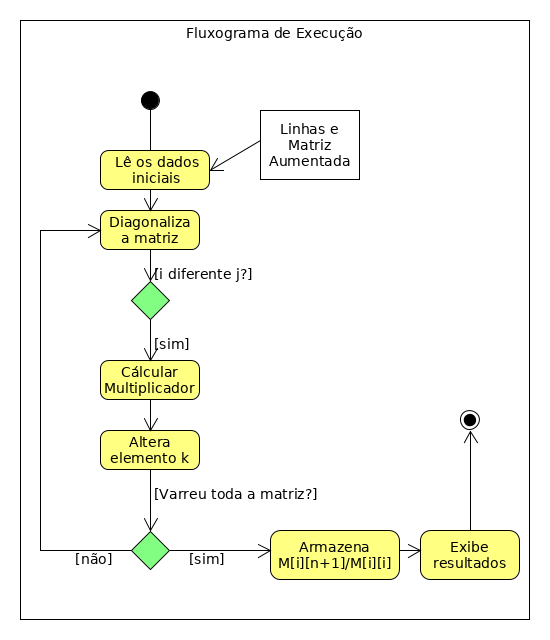
\includegraphics[width=10cm]{figuras/fluxograma.png}\\
  \caption{Fluxo de execução da solução}\label{fig:fluxo}
\end{figure}

A solução elaborada neste relatório funciona da seguinte maneira. É necessário inserir a quantiade de linhas
do sistema de equações lineares, em formato de matriz aumentada, que se quer resolver. Após isso o programa
solicitará a inserção dos elementos de cada uma das linhas da matriz. Após completar a matriz de entrada o
sistema irá fazer a diagonalização de acordo com o método de eliminação de Gaus-Jordan. Onde caso os índices
i e j sejam diferentes, ou seja não fazem parte da diagonal principal, será aplicado o algoritmo de eliminação.
Após haver apenas os elementos da diagonal principal, o método de solução se torna direto e com isso é possível
encontrar os valores da incógnitas que se busca. As limitações do programa são entradas de matrizes de no máximo
10x10 e apenas para equações lineares.

\newpage
\section{Código Fonte}

\lstinputlisting[language=C]{../solution/m3.c}

\newpage
\section{Resultados e discussões}

Nesta seção discutiremos os resultados obtidos após a execução.

\begin{figure}[!h]
  \centering
  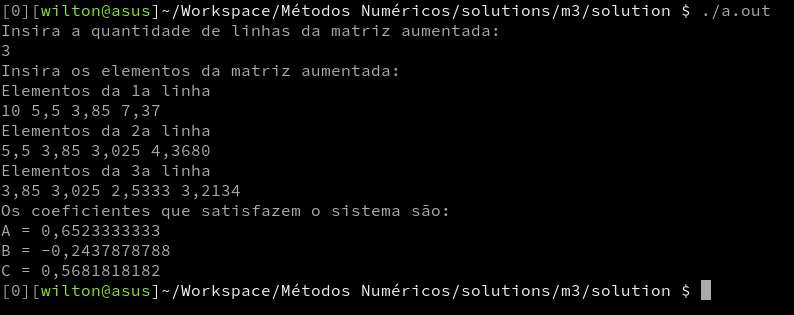
\includegraphics[width=15cm]{figuras/printx.png}\\
  \caption{Resultado da execução do programa}\label{fig:printx}
\end{figure}
Após a execução do programa obtemos os valores dos coeficientes que resulta no seguinte polinômio:
\begin{eqnarray}\label{eq:polinomio}
  C(x) = 0,6523 - 0,2438x + 0,5682x^2
\end{eqnarray}
O resultado encontrado a partir da solução proposta é condizente. Pois ao fazermos a comparação dos valores iniciais com os obtidos através da equação~\eqref{eq:polinomio} encontramos valores bem próximos uns dos outros, como pode ser visto na tabela abaixo:

\begin{table}[h]
  \centering
  \vspace{0.5cm}
  \begin{tabular}{|r|r|r|r|r|r|r|r|r|r|r|}
    \hline
    \multicolumn{11}{|c|}{Valores iniciais do experimento} \\
    \hline
      $\frac{A}{A_1}$ & 0.10 & 0.20 & 0.30 & 0.40 & 0.50 & 0.60 & 0.70 & 0.80 & 0.90 & 1.00\\
    \hline
      $C$ & 0.62 & 0.63 & 0.64 & 0.66 & 0.68 & 0.71 & 0.76 & 0.81 & 0.89 & 1.00\\
    \hline
    \multicolumn{11}{|c|}{Valores obtidos após o método} \\
    \hline
      $\frac{A}{A_1}$ & 0.10 & 0.20 & 0.30 & 0.40 & 0.50 & 0.60 & 0.70 & 0.80 & 0.90 & 1.00\\
    \hline
      $C$ & 0.63 & 0.63 & 0.63 & 0.65 & 0.67 & 0.71 & 0.76 & 0.82 & 0.89 & 0.98\\
    \hline
  \end{tabular}
  \caption{Valores experimentais e de regressão}
\end{table}

\newpage
E também graficamente, como é mostrado abaixo:
\begin{figure}[!h]
  \centering
  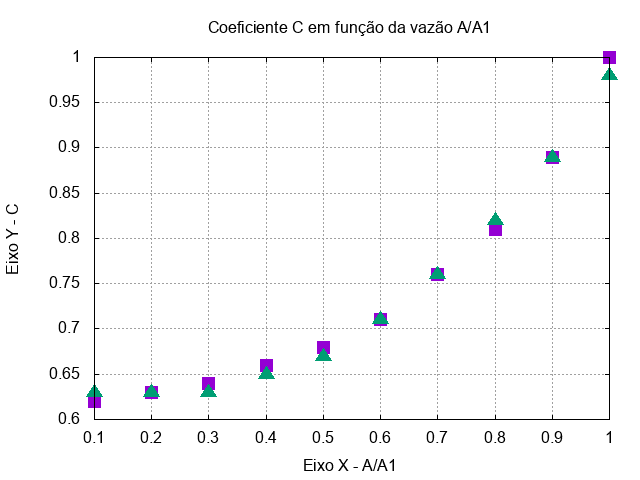
\includegraphics[width=12cm]{figuras/coef.png}\\
\end{figure}

Sendo assim, o objetivo proposto no início do relatório foi satisfatoriamente alcançado.

\newpage
\section{Ferramentas}
Todas as ferramentas utilizadas neste relatório são ferramentas open source (software livre).
Permitindo assim que qualquer um possa reproduzir e contestar as afirmações presentes neste documento.

\begin{enumerate}
  \item Arch Linux (\url{https://www.archlinux.org})
    \begin{itemize}
      \item Sistema operacional utilizado.
    \end{itemize}
  \item GCC (\url{https://gcc.gnu.org})
    \begin{itemize}
      \item Compilador de C utilizado para compilar a solução.
    \end{itemize}
  \item Python (\url{https://www.python.org})
    \begin{itemize}
      \item Linguagem de programação utilizada para conferir os valores da solução.
    \end{itemize}
  \item vim (\url{http://www.vim.org})
    \begin{itemize}
      \item Editor de texto.
    \end{itemize}
  \item \LaTeX~(\url{https://www.latex-project.org})
    \begin{itemize}
      \item Sistema tipográfico de alta qualidade (utilizado para elaborar o relatório).
    \end{itemize}
  \item Gnuplot (\url{http://www.gnuplot.info})
    \begin{itemize}
      \item Utilitário de representação gráfica (utilizado para plotagem do gráfico).
    \end{itemize}
  \item UMLet (\url{http://www.umlet.com})
    \begin{itemize}
      \item Ferramenta de UML (utilizado para criar o fluxo de execução).
    \end{itemize}
  \item Shutter (\url{http://shutter-project.org})
    \begin{itemize}
      \item Programa de captura de tela (utilizado para capturar os resultados).
    \end{itemize}
\end{enumerate}

%%%%%%%%%%%%%%%%%%%%%%%%%%%%%%%%%%%%%%%%%%%%%%%%%%%%%%%%%%%%%%%%%%%%%%%%%%%%%%%%%%%%%%%%%

\end{document}
